% !TeX root = main.tex
\chapter{Published software}\label{app:tech}

As part of the research presented in this theis, we developed several systems for semantic speech editing and audio
visualization. We have since published these systems as open-source software for others to use. This chapter outlines
the technical details behind the implementation of these systems, including notes on how we approached the more
challenging aspects of design.

\section{Dialogger}\label{sec:dialogger}

Dialogger is a semantic audio and video editor that enables the navigation and editing of media recordings using a
text-based interface. The design and operation of Dialogger is outlined in Section~\ref{sec:paper-screen-design}. We
have published the system as open-source software under an Apache 2.0 licence at the following URL:
\url{https://github.com/bbc/dialogger}

%Requirements:
%Correction (i.e. text editing)
%while retaining timestamps
%Editing (i.e. audio editing)
%Live preview of edits
%Display/edit speaker segments
%Display timestamps
%Export EDL

%Solution:
%Use CKEditor for text editing with restricted functionality
  %No cut/copy/paste or dragging
  %Replace only
  %Selections jump to start/end of words
  %Generate new timestamps when replacing >1 word
%Edit audio using bold/underline
%Use HTML5-video-compositor for preview
%JSON->HTML, HTML->JSON
%JSON->EDL

Dialogger includes features for playback and navigation of media using a transcript, transcript editing, export of edit
decision lists (EDLs), user accounts and media asset management. Our system does not include an ASR system, media
format converter or media file export, however these can easily be integrated using the instructions in the user guide.

\subsection{System overview}

The structure and data flow of Dialogger is shown in Figure~\ref{fig:dialogger-flow}. We divided our system into a
presentation layer (front end) and a data management layer (back end). The front end used HTML, CSS and Javascript so
that the system could be accessed through a web browser.  We used \textit{Semantic UI} as a user interface framework,
\textit{Backbone} as a model-view-controller framework and \textit{Dropzone} to handle file uploads.

\begin{figure}[t]
\centering
  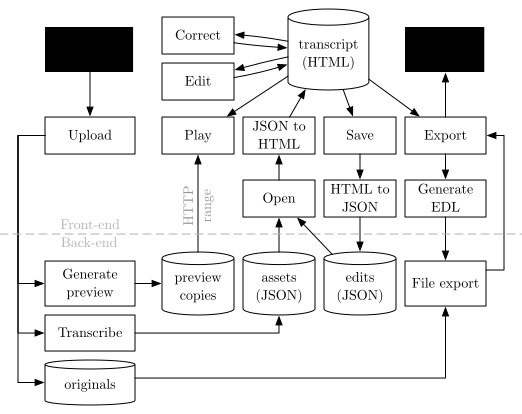
\includegraphics[width=.8\textwidth]{figs/dialogger-flow-diagram.pdf}
  \caption{Flow diagram of the Dialogger system. Excluded components are shaded.}
  \label{fig:dialogger-flow}
\end{figure}

For the back end, we used \textit{Node.js} and \textit{Express} as our framework, and \textit{MongoDB} for our
database. We authenticated users using \textit{Passport.js}, logged errors using \textit{Bunyan} and used
\textit{Mimovie} to extract metadata from uploaded media files.

\subsection{Word processing}

We included word processing functionality in Dialogger to allow users to navigate the speech, correct mistakes in the
transcript and mark up edit decisons.  We used the \textit{CKEditor} Javascript library as the basis for the word
processing functionality in our interface.

\paragraph{Timestamps}
In addition to the requirements of a normal word processor, our system had a unique requirement for each word to
include a hidden timestamp, and for that timestamp to be retained throughout the editing process.  We achieved this by
using HTML formatting for the text, adding a HTML tag to each word, and including the timestamp as an attribute in the 
tag. This linked the timestamps to the words, but certain edit actions created problems, as explained below.

\paragraph{Split words}
Traditional word processors allow users to select text with the granularity of individual characters. This caused an
issue where words could be split by cutting, moving or replacing only part of a word. To avoid this problem, we
restricted editing to word level-granularity by automatically moving the user's selection to the start and end of any
selected words.

\paragraph{Joined words}
Occassionally, ASR systems will transcribe a single word as two words. When the user selects both words and types a
replacement, then both words are replaced and their timestamps are lost. To avoid this, we added logic that detected
this behaviour and created a new word with the start time of the first word and the end time of the last word.

\paragraph{Re-ordering}
Word processing gives users the freedom to move and edit words freely.  However, when text is moved around it becomes
very difficult for the user to keep track of the original location and order of the words. This is a problem with audio
editing as some edits sound unacceptable, so users will often want to adjust the edit.
Our solution was to retain the sequence of the words so that their original positions were retined. This prevented
re-ordering of the words, but this could be handled later by a DAW.  We implemented this restriction by disabling cut,
copy, paste and drag-and-drop.

\subsection{Media integration}

We used timestamps to link each word in the transcript to a segment of source media.  To integrate the transcript with
the media, we built systems to generate an edit decisions list (EDL) based on the user's annotations, instantly preview
those edits in the browser, and allow the user to download a copy of the final edit.

\paragraph{EDL generation}
In addition to including the start and end timestamp of each word in their HTML tag, we included the timestamp of the
next word. To find edit points, we simply looked for any difference in the predicted and actual timestamp of a word.
We could then generate an EDL by filtering words based on their annotation, then looking for edit points. However, this
approach relies on the words being in their original sequence.

\paragraph{Preview}
We wanted users to be able to preview their edits to quickly hear whether they sound acceptable or not.  To implement
this feature, we used \textit{HTML5 Video Compositor} --- a media composition engine that can play edit decision lists
in the browser.

Content can be dynamically appended to the EDL as it's playing to create interactive and responsive content.

In video editing terms an EDL defines the points at which to cut and assemble video sources. VideoCompositor uses a simple JSON based EDL to describe how to cut and assemble HTML5 video sources, images, and WebGL contexts, it also provides a framework for performing shader based compositing operations (i.e cross-fades, green-screen).



\paragraph{Export}


\clearpage
\section{Vampeyer}\label{sec:vampeyer}
The direction of the research in this project centres around turning audio data into image data. There is already some
software that visualizes audio and audio features in a number of ways, notably Sonic Visualiser \citep{Cannam2010}.
However, the visualization algorithms are always hard-coded into the program, making prototyping of new methods
prohibitively difficult.

\subsection{Design}
A system of software was developed for visualizing audio in order to allow flexibility while maintaining consist inputs
and outputs. It was designed to expand on existing systems for audio analysis so to avoid duplication of effort and to
allow modularisation of algorithms.

The system was developed as a plugin framework with clearly defined inputs and outputs. It is based on the existing
Vamp plugin framework, developed by Queen Mary University of London \citep{Cannam2010}, which analyses audio data and
outputs frame-- or time-based features. The visualization plugin is designed to take these features and produce a
bitmap image. An outline of the system design is shown in Figure~\ref{fig:vampeyer}.

\begin{figure}[ht]
  \centering
  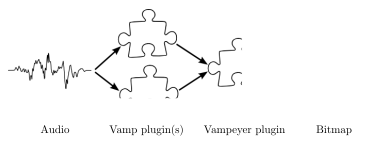
\includegraphics[width=0.8\textwidth]{figs/vampeyer.pdf}
  \caption{High-level system diagram of the Vampeyer visualization framework}
  \label{fig:vampeyer}
\end{figure}

The visualization plugin defines which Vamp plugin outputs it requires, including the block/step size and parameters.
At least one Vamp plugin is required, but there is no restriction of the number of different Vamp plugins that can be
used.

Both frameworks are written in C++ which allows for a fast processing time.  This is important for situations where
audio has to be processed on-the-fly, such as for exploring an archive without having to pre-process everything in it.
The plugins are compiled into shared libraries, so they can easily be distributed without users having to recompile
locally and integrated into third-party software.

\subsection{Implementation}
A C++ header file was created which implements the design.  Five data structures are also defined which define how data
should be sent and returned from the functions.

{\singlespacing
\begin{itemize}
  \item \texttt{VampParameter} is a name/value pair used to store a parameter
  \item \texttt{VampParameterList} is a vector of \texttt{VampParameter}s
  \item \texttt{VampPlugin} stores the name of a Vamp plugin along with a\\
    \texttt{VampParameterList} and the preferred block and step sizes
  \item \texttt{VampOutput} stores a \texttt{VampPlugin} and output name
  \item \texttt{VampOutputList} is a vector of \texttt{VampOutput}s
\end{itemize}
}

Two primary functions are used to define the input audio features and their conversion to a bitmap.

\begin{itemize}
  \item \texttt{getVampPlugins} returns a \texttt{VampOutputList} variable that contains a list of Vamp plugin outputs
    which must be provided as input
  \item \texttt{ARGB} takes the Vamp plugin output data as a \texttt{Vamp::FeatureSet} variable, the sample rate of the
    audio and the desired width and height. It returns a bitmap image formatted in 32-bit ARGB format (alpha, red,
    green, blue).
\end{itemize}

A number of example plugins were written to demonstrate the capabilities of this approach, and to act as useful pieces
of software in their own right.  These include a standard waveform, waveform colourised by low energy ratio (see
Section~\ref{sec:studywaveform}), waveform colourised by spectral centroid (identical to Freesound) and an MFCC grid
visualization with waveform overlay.

The plugins need to be run by a host program which reads the audio data, processes it using the Vamp plugins, sends
their output to the visualization plugin and then writes the image data. Such a program was written as a command-line
tool that can either display the image in a window or write it to disk as a PNG-encoded file. This makes it useful for
both prototyping and for back-end processing on a server, for example.

\clearpage
\section{BeatMap}\label{sec:beatmap}

\begin{figure}[h]
\centering
  \includegraphics[width=\textwidth]{figs/beatmap.png}
  \caption{Example user interface that uses the BeatMap library.}
  \label{fig:beatmap}
\end{figure}
